\documentclass[tikz,border=15pt]{standalone}
\usepackage{tikz}
\usepackage{xcolor}
\usetikzlibrary{arrows.meta,calc}

\definecolor{bgcolor}{RGB}{15,23,42}
\definecolor{cardbg}{RGB}{30,41,59}
\definecolor{cardborder}{RGB}{51,65,85}
\definecolor{linkorange}{RGB}{234,88,12}
\definecolor{linkborder}{RGB}{124,45,18}
\definecolor{jointsilver}{RGB}{203,213,225}
\definecolor{jointdark}{RGB}{100,116,139}
\definecolor{metaldark}{RGB}{51,65,85}
\definecolor{rotblue}{RGB}{56,189,248}
\definecolor{rotyellow}{RGB}{250,204,21}
\definecolor{grippergreen}{RGB}{34,197,94}
\definecolor{grippertarget}{RGB}{56,189,248}
\definecolor{slategray}{RGB}{148,163,184}

\begin{document}
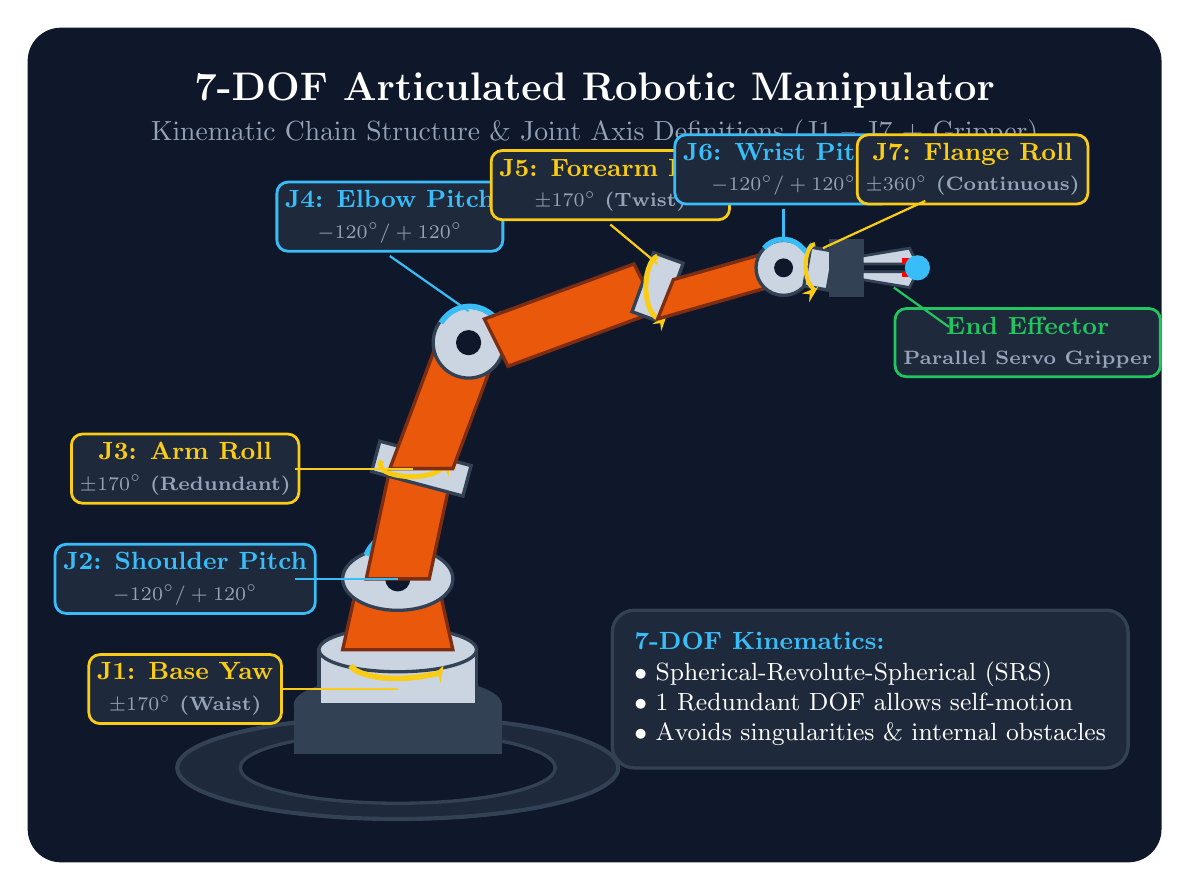
\begin{tikzpicture}[
    >={Stealth[length=6pt, width=4pt]}
]

% Background Card
\fill[rounded corners=12pt, fill=bgcolor] (-7.2,-5.4) rectangle (7.2,5.2);

% Title & Header
\node[text=white, font=\Large\bfseries] at (0, 4.4) {7-DOF Articulated Robotic Manipulator};
\node[text=slategray, font=\normalsize] at (0, 3.85) {Kinematic Chain Structure \& Joint Axis Definitions (J1 -- J7 + Gripper)};

% Pedestal Floor Mounting
\fill[cardbg, draw=cardborder, line width=1.5pt] (-2.5, -4.2) ellipse (2.8cm and 0.65cm);
\fill[bgcolor, draw=cardborder, line width=1.2pt] (-2.5, -4.2) ellipse (2.0cm and 0.45cm);

% 1. BASE & J1 (Base Yaw)
\fill[metaldark, draw=cardborder, line width=1.2pt] (-3.8, -4.0) rectangle (-1.2, -3.4);
\fill[metaldark, draw=cardborder, line width=1.2pt] (-2.5, -3.4) ellipse (1.3cm and 0.35cm);
\fill[jointsilver, draw=cardborder, line width=1.2pt] (-3.5, -3.4) rectangle (-1.5, -2.7);
\fill[jointsilver, draw=cardborder, line width=1.2pt] (-2.5, -2.7) ellipse (1.0cm and 0.28cm);

% J1 Rotation Arrow
\draw[rotyellow, line width=2pt, ->] (-3.1, -2.9) arc (190:350:0.6 and 0.2);

% 2. J2 (Shoulder Pitch)
\fill[linkorange, draw=linkborder, line width=1.2pt] (-3.2, -2.7) -- (-1.8, -2.7) -- (-2.0, -1.8) -- (-3.0, -1.8) -- cycle;
\fill[jointsilver, draw=cardborder, line width=1.2pt] (-2.5, -1.8) ellipse (0.7cm and 0.4cm);
\fill[bgcolor] (-2.5, -1.8) circle (0.16cm);
\draw[rotblue, line width=2pt, ->] (-2.9, -1.5) arc (160:20:0.42);

% 3. LINK 1 & J3 (Arm Roll)
\fill[linkorange, draw=linkborder, line width=1.2pt] (-2.9, -1.8) -- (-2.1, -1.8) -- (-1.8, -0.4) -- (-2.6, -0.4) -- cycle;
% J3 Roll Joint
\fill[jointsilver, draw=cardborder, line width=1.2pt, rotate around={-15:(-2.2, -0.4)}] (-2.8, -0.6) rectangle (-1.6, -0.2);
\draw[rotyellow, line width=1.8pt, ->] (-2.7, -0.3) arc (160:380:0.4 and 0.15);

% Upper arm to elbow
\fill[linkorange, draw=linkborder, line width=1.2pt] (-2.6, -0.4) -- (-1.8, -0.4) -- (-1.2, 1.2) -- (-2.0, 1.2) -- cycle;

% 4. J4 (Elbow Pitch)
\fill[jointsilver, draw=cardborder, line width=1.2pt] (-1.6, 1.2) circle (0.45cm);
\fill[bgcolor] (-1.6, 1.2) circle (0.16cm);
\draw[rotblue, line width=2pt, ->] (-1.95, 1.45) arc (150:20:0.42);

% 5. LINK 2 & J5 (Forearm Roll)
\fill[linkorange, draw=linkborder, line width=1.2pt] (-1.4, 1.5) -- (-1.1, 0.9) -- (0.8, 1.6) -- (0.5, 2.2) -- cycle;
% J5 Joint
\fill[jointsilver, draw=cardborder, line width=1.2pt, rotate around={-20:(0.8, 1.9)}] (0.6, 1.5) rectangle (1.0, 2.3);
\draw[rotyellow, line width=1.8pt, ->] (0.8, 2.3) arc (100:300:0.18 and 0.4);

% Forearm to wrist
\fill[linkorange, draw=linkborder, line width=1.2pt] (1.0, 2.0) -- (0.8, 1.5) -- (2.2, 1.9) -- (2.4, 2.4) -- cycle;

% 6. J6 (Wrist Pitch)
\fill[jointsilver, draw=cardborder, line width=1.2pt] (2.4, 2.15) circle (0.35cm);
\fill[bgcolor] (2.4, 2.15) circle (0.12cm);
\draw[rotblue, line width=1.8pt, ->] (2.15, 2.4) arc (140:10:0.32);

% 7. J7 (Flange Roll) & GRIPPER
\fill[jointsilver, draw=cardborder, line width=1.2pt, rotate around={-10:(2.8, 2.15)}] (2.7, 1.9) rectangle (3.0, 2.4);
\draw[rotyellow, line width=1.5pt, ->] (2.8, 2.45) arc (90:290:0.12 and 0.28);

% Gripper Body & Fingers
\fill[metaldark, draw=cardborder, line width=1.2pt] (3.0, 1.8) rectangle (3.4, 2.5);
\fill[jointsilver, draw=cardborder, line width=1pt] (3.4, 2.3) -- (4.0, 2.4) -- (4.1, 2.2) -- (3.4, 2.2) -- cycle;
\fill[red] (3.9, 2.2) rectangle (4.1, 2.27);
\fill[jointsilver, draw=cardborder, line width=1pt] (3.4, 2.0) -- (4.0, 1.9) -- (4.1, 2.1) -- (3.4, 2.1) -- cycle;
\fill[red] (3.9, 2.03) rectangle (4.1, 2.1);
\fill[grippertarget] (4.1, 2.15) circle (0.16cm);

% LABELS & CALLOUTS
% J1
\node[fill=cardbg, draw=rotyellow, line width=1pt, rounded corners=4pt, text=rotyellow, font=\small\bfseries, align=center, inner sep=3pt] at (-5.2, -3.2) {
    J1: Base Yaw\\
    \textcolor{slategray}{\scriptsize $\pm 170^\circ$ (Waist)}
};
\draw[rotyellow, line width=0.8pt] (-4.0, -3.2) -- (-2.5, -3.2);

% J2
\node[fill=cardbg, draw=rotblue, line width=1pt, rounded corners=4pt, text=rotblue, font=\small\bfseries, align=center, inner sep=3pt] at (-5.2, -1.8) {
    J2: Shoulder Pitch\\
    \textcolor{slategray}{\scriptsize $-120^\circ / +120^\circ$}
};
\draw[rotblue, line width=0.8pt] (-3.8, -1.8) -- (-2.5, -1.8);

% J3
\node[fill=cardbg, draw=rotyellow, line width=1pt, rounded corners=4pt, text=rotyellow, font=\small\bfseries, align=center, inner sep=3pt] at (-5.2, -0.4) {
    J3: Arm Roll\\
    \textcolor{slategray}{\scriptsize $\pm 170^\circ$ (Redundant)}
};
\draw[rotyellow, line width=0.8pt] (-3.8, -0.4) -- (-2.3, -0.4);

% J4
\node[fill=cardbg, draw=rotblue, line width=1pt, rounded corners=4pt, text=rotblue, font=\small\bfseries, align=center, inner sep=3pt] at (-2.6, 2.8) {
    J4: Elbow Pitch\\
    \textcolor{slategray}{\scriptsize $-120^\circ / +120^\circ$}
};
\draw[rotblue, line width=0.8pt] (-2.6, 2.3) -- (-1.6, 1.6);

% J5
\node[fill=cardbg, draw=rotyellow, line width=1pt, rounded corners=4pt, text=rotyellow, font=\small\bfseries, align=center, inner sep=3pt] at (0.2, 3.2) {
    J5: Forearm Roll\\
    \textcolor{slategray}{\scriptsize $\pm 170^\circ$ (Twist)}
};
\draw[rotyellow, line width=0.8pt] (0.2, 2.7) -- (0.8, 2.2);

% J6
\node[fill=cardbg, draw=rotblue, line width=1pt, rounded corners=4pt, text=rotblue, font=\small\bfseries, align=center, inner sep=3pt] at (2.4, 3.4) {
    J6: Wrist Pitch\\
    \textcolor{slategray}{\scriptsize $-120^\circ / +120^\circ$}
};
\draw[rotblue, line width=0.8pt] (2.4, 2.9) -- (2.4, 2.5);

% J7
\node[fill=cardbg, draw=rotyellow, line width=1pt, rounded corners=4pt, text=rotyellow, font=\small\bfseries, align=center, inner sep=3pt] at (4.8, 3.4) {
    J7: Flange Roll\\
    \textcolor{slategray}{\scriptsize $\pm 360^\circ$ (Continuous)}
};
\draw[rotyellow, line width=0.8pt] (4.2, 3.0) -- (2.9, 2.4);

% Gripper
\node[fill=cardbg, draw=grippergreen, line width=1pt, rounded corners=4pt, text=grippergreen, font=\small\bfseries, align=center, inner sep=3pt] at (5.5, 1.2) {
    End Effector\\
    \textcolor{slategray}{\scriptsize Parallel Servo Gripper}
};
\draw[grippergreen, line width=0.8pt] (4.5, 1.4) -- (3.8, 1.9);

% Kinematics Info Card (Bottom Right)
\node[fill=cardbg, draw=cardborder, line width=1.2pt, rounded corners=8pt, text=white, font=\small, align=left, inner sep=8pt] at (3.5, -3.2) {
    \textbf{\textcolor{rotblue}{7-DOF Kinematics:}}\\
    $\bullet$ Spherical-Revolute-Spherical (SRS)\\
    $\bullet$ 1 Redundant DOF allows self-motion\\
    $\bullet$ Avoids singularities \& internal obstacles
};

\end{tikzpicture}
\end{document}
